% ============================================================
% Electoral Judicialization and Municipal Competition in Brazil
% Beamer presentation — Nara Lívia Morais (FEA-USP)
%
% Compile with: pdflatex (twice)
% ============================================================

\documentclass[aspectratio=169,10pt]{beamer}

% ---- Theme ----
\usetheme{default}
\useinnertheme{rectangles}
\setbeamertemplate{navigation symbols}{}
\setbeamertemplate{footline}[frame number]

% ---- Packages ----
\usepackage{booktabs}
\usepackage{amsmath,amssymb}
\usepackage{graphicx}
\usepackage{xcolor}
\usepackage{tikz}
\usetikzlibrary{arrows.meta,shapes.geometric,positioning,fit,backgrounds}
\usepackage{array}
\usepackage{multirow}
\usepackage{tabularx}
\usepackage{hyperref}
\usepackage[utf8]{inputenc}

% ---- Colors ----
\definecolor{myblue}{RGB}{0,90,156}
\definecolor{mydark}{RGB}{55,55,55}
\definecolor{mylight}{RGB}{220,230,242}
\definecolor{myred}{RGB}{180,30,30}
\definecolor{mygreen}{RGB}{0,120,60}
\definecolor{mygray}{RGB}{130,130,130}

\setbeamercolor{frametitle}{bg=myblue,fg=white}
\setbeamercolor{title}{fg=white,bg=myblue}
\setbeamercolor{subtitle}{fg=mylight,bg=myblue}
\setbeamercolor{author in head/foot}{fg=white,bg=myblue!80}
\setbeamercolor{structure}{fg=myblue}
\setbeamercolor{alerted text}{fg=myred}
\setbeamercolor{block title}{bg=myblue!20,fg=myblue}
\setbeamercolor{block body}{bg=myblue!5}
\setbeamercolor{block title alerted}{bg=myred!20,fg=myred}
\setbeamercolor{block body alerted}{bg=myred!5}
\setbeamerfont{frametitle}{size=\normalsize,series=\bfseries}

% ---- Column types ----
\newcolumntype{L}[1]{>{\raggedright\arraybackslash}p{#1}}
\newcolumntype{C}[1]{>{\centering\arraybackslash}p{#1}}
\newcolumntype{R}[1]{>{\raggedleft\arraybackslash}p{#1}}

% ---- Custom commands ----
\newcommand{\bZ}{\mathit{Z}_{m}^{\textsc{b}}}
\newcommand{\todo}[1]{\textcolor{mygray}{\textit{[#1]}}}
\newcommand{\pos}[1]{\textcolor{mygreen}{\textbf{#1}}}
\newcommand{\negt}[1]{\textcolor{myred}{\textbf{#1}}}
\newcommand{\ns}[1]{\textcolor{mydark}{#1}}
\newcommand{\tick}{{\color{mygreen}$\checkmark$}}
\newcommand{\cross}{{\color{myred}$\times$}}

% ---- Title info ----
\title{Electoral Judicialization and\\Municipal Competition in Brazil}
\subtitle{Evidence from a Bartik Shift-Share Instrument}
\author{Nara Lívia Morais}
\institute{FEA--USP}
\date{\today}

% ============================================================
\begin{document}
% ============================================================

\maketitle

% ============================================================
\section{Motivation}
% ============================================================

\begin{frame}{Does Judicial Intervention Shape Electoral Competition?}
\begin{columns}[T]
\begin{column}{0.58\textwidth}
\textbf{Research question:}\\
Does pre-election judicial intervention causally affect the competitive dynamics of mayoral races?
\bigskip

\textbf{The mechanism:}
\begin{itemize}
  \item Candidates face adversarial lawsuits \emph{before} election day
  \item Lawsuits impose legal costs, reputational exposure, and campaign disruption
  \item This could deter entry, shift vote shares, and alter voter behavior
\end{itemize}
\bigskip

\textbf{The challenge:}\\
Close races \emph{attract} more lawsuits --- endogeneity runs in both directions
\end{column}
\begin{column}{0.40\textwidth}
\begin{block}{This Paper}
  \begin{itemize}
    \item 5,560 Brazilian municipalities
    \item 2020 and 2024 mayoral elections
    \item TSE administrative data
    \item Identification: \textbf{Bartik shift-share IV} (F\,$\approx$\,19.6)
  \end{itemize}
\end{block}
\begin{alertblock}{Key Findings}
  \footnotesize
  Adversarial judicialization $\uparrow$ significantly raises the blank vote rate ($+$1.3\,pp, $p=0.018$). Candidate pool contracts (directional). Competition and turnout: precise nulls after tF correction.
\end{alertblock}
\end{column}
\end{columns}
\end{frame}


\begin{frame}{Why Brazil? Why Municipalities?}
\begin{columns}[T]
\begin{column}{0.55\textwidth}
\textbf{Brazil's Electoral Justice System:}
\begin{itemize}
  \item \emph{Tribunal Superior Eleitoral} (TSE) + 27 \emph{Tribunais Regionais Eleitorais} + 2,800+ first-instance zones
  \item Adjudicates eligibility, campaign finance, and conduct \emph{before} election day
  \item Among the world's most active electoral court systems
  \item Rich variation in topic mix across municipalities, states, and cycles
\end{itemize}
\end{column}
\begin{column}{0.43\textwidth}
\begin{block}{Municipal Setting}
  \begin{itemize}
    \item 5,570 simultaneous contests $=$ large cross-section
    \item Homogeneous office: directly elected mayor
    \item Uniform electoral rules (CF Art.~29)
    \item Comparable competitive dynamics across units
  \end{itemize}
\end{block}
\begin{block}{Two Election Cycles}
  2020 (Nov 15) $\to$ \textbf{shares}\\
  2024 (Oct 6) $\to$ \textbf{treatment + outcomes}
\end{block}
\end{column}
\end{columns}
\end{frame}


\begin{frame}{Road Map}
\tableofcontents
\end{frame}


% ============================================================
\section{Institutional Background}
% ============================================================

\begin{frame}{Brazil's Electoral Justice System}
\begin{columns}[T]
\begin{column}{0.55\textwidth}
\textbf{Three-tier judicial structure:}
\begin{enumerate}
  \item \textbf{Zona Eleitoral (ZE)} --- first instance; 2,800+ nationwide
  \item \textbf{Tribunal Regional Eleitoral (TRE)} --- 27 state appellate courts
  \item \textbf{Tribunal Superior Eleitoral (TSE)} --- national apex
\end{enumerate}
\bigskip
\textbf{Pre-election jurisdiction:}
\begin{itemize}
  \item Candidate registration challenges (\emph{impugna\c{c}\~{a}o})
  \item Abuse of economic/political power
  \item Campaign finance violations
  \item Prohibited propaganda; vote-buying
  \item Conduct prohibitions (\emph{conduta vedada})
\end{itemize}
\end{column}
\begin{column}{0.43\textwidth}
\begin{block}{Election Timeline}
  \footnotesize
  \begin{enumerate}
    \item Candidate registration (August)
    \item \textbf{Pre-election lawsuits} (Aug--Oct)
    \item \textbf{Election Day} (Oct/Nov)
    \item Post-election proceedings
    \item Cassation if ruling goes against winner
  \end{enumerate}
\end{block}
\bigskip
\footnotesize
\textbf{2020:} Election day = November 15\\
\textbf{2024:} Election day = October 6\\[4pt]
We use only cases filed \emph{before} these dates.
\end{column}
\end{columns}
\end{frame}


\begin{frame}{What Lawsuits Do --- and Who Files Them}
\begin{columns}[T]
\begin{column}{0.55\textwidth}
\textbf{Effects on targeted candidates:}
\begin{itemize}
  \item \textbf{Candidacy at risk:} court may rule ineligible before election day
  \item \textbf{Reputational cost:} public filing, media coverage, social stigma
  \item \textbf{Resource diversion:} legal defense competes with campaigning
  \item \textbf{Quality signal to voters:} a respondent may be perceived as ethically challenged --- or as a victim of political harassment
\end{itemize}
\bigskip
\textbf{Who files?}\\
Opposing candidates, parties, \emph{Ministério Público Eleitoral}, any citizen
\end{column}
\begin{column}{0.43\textwidth}
\begin{alertblock}{Treatment Variable}
  \textbf{Adversarial competition-relevant cases:}
  \begin{itemize}
    \item Mayoral candidate is the \emph{respondent}
    \item Filed before election day
    \item Substantive challenge (adversarial class and subject — not administrative)
  \end{itemize}
  \bigskip
  \textbf{Measurement:}\\
  $\Delta\log(1+\text{lawsuits}_{m})$\\from 2020 to 2024
\end{alertblock}
\end{column}
\end{columns}
\end{frame}


\begin{frame}{Administrative vs.\ Adversarial Electoral Litigation}
\begin{columns}[T]
\begin{column}{0.57\textwidth}
Not all electoral case subjects involve genuine legal challenges to candidates:
\bigskip
\begin{description}
  \item[\textbf{Candidacy Registration (RRC):}] Automatically generated for \emph{every} registered candidacy. No plaintiff, no adversarial content, no legal risk. Purely administrative.
  \medskip
  \item[\textbf{Coalition Slate Registration (DRAP):}] Filed by each party before every election; mandatory under Art.~6, Lei~9.504/1997. Universal coverage ($>$97\% of municipalities).
  \medskip
  \item[\textbf{Adversarial challenges:}] Filed against a specific candidate's conduct, eligibility, or campaign behaviour by opponents, the Electoral Public Prosecutor (\emph{MPE}), or citizens. These constitute genuine judicial intervention.
\end{description}
\end{column}
\begin{column}{0.41\textwidth}
\begin{block}{Case Volume (2020)}
  \footnotesize
  \renewcommand{\arraystretch}{1.2}
  \begin{tabular}{lrc}
    \toprule
    Type & Volume & Included? \\
    \midrule
    Candidacy registration (RRC) & $\sim$994k & \cross \\
    Coalition registration (DRAP) & $\sim$137k & \cross \\
    Admin.\ procedural classes & various & \cross \\
    \midrule
    Eligibility challenges & & \tick \\
    Abuse of power & & \tick \\
    Campaign conduct & & \tick \\
    Propaganda violations & & \tick \\
    Document/information offenses & & \tick \\
    \bottomrule
  \end{tabular}
\end{block}
\medskip
\footnotesize\textit{Adversarial filter applied at data construction stage (class and subject exclusions).}
\end{column}
\end{columns}
\end{frame}


\begin{frame}{Pre-Election Timing Restriction}
\begin{itemize}
  \item \textbf{Restriction:} we keep only cases filed \textit{strictly before} election day:
  \[
    \text{filing date} < \text{election date}
  \]
  \medskip
  \item \textbf{Rationale:} only pre-election cases can plausibly affect competitive dynamics through legal costs, reputational signaling, or candidacy threats
  \medskip
  \item Post-election \emph{cassa\c{c}\~{a}o} proceedings determine whether the \emph{realized winner} is removed --- a distinct phenomenon that could reverse causality
  \medskip
  \item Applied identically to both the 2020 baseline (for shares) and the 2024 measurement (for treatment)
  \medskip
  \item \textbf{Future robustness:} \todo{test with $>$30\,days before election day to address late strategic filings}
\end{itemize}
\end{frame}


\begin{frame}{The Endogeneity Problem}
\begin{columns}[T]
\begin{column}{0.55\textwidth}
\textbf{OLS is likely biased:}
\bigskip
\begin{enumerate}
  \item \textbf{Competition $\to$ lawsuits}\\
  Close races attract more suits; positive confound with competitiveness
  \medskip
  \item \textbf{Vulnerability $\to$ lawsuits}\\
  Incumbent weakness invites challengers to file; negative confound with incumbency
  \medskip
  \item \textbf{Unobservables}\\
  Local political culture, lawyer density, party intensity --- correlated with both
\end{enumerate}
\bigskip
Direction of bias: \textbf{ambiguous}
\end{column}
\begin{column}{0.43\textwidth}
\begin{alertblock}{Identification Need}
  We need exogenous variation in the \emph{level} of judicialization independent of the municipality's own 2024 competitive dynamics.
\end{alertblock}
\bigskip
\begin{block}{Our Strategy}
  \textbf{Bartik shift-share IV:}\\
  Predicted 2024 lawsuits from the municipality's 2020 topic mix $\times$ state-level topic growth --- a source of variation the municipality does not drive.
  \medskip\\
  \footnotesize Theoretical framework: Helmke \& Staton (2011) — litigation waves in Latin America driven by institutional and strategic diffusion at the supra-municipal level.
\end{block}
\end{column}
\end{columns}
\end{frame}


% ============================================================
\section{Data Construction}
% ============================================================

\begin{frame}{Data Pipeline Overview}
\begin{center}
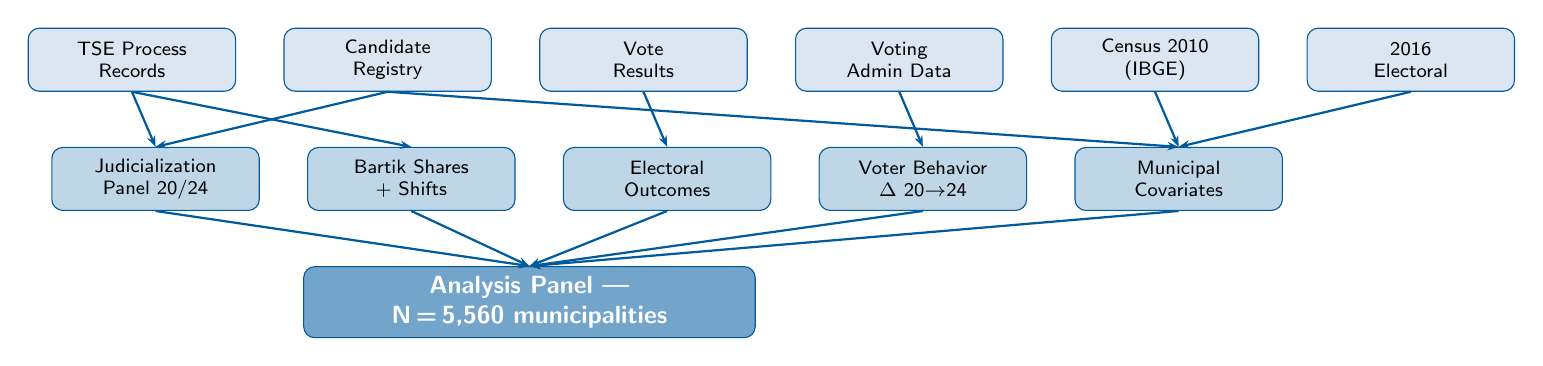
\begin{tikzpicture}[
    node distance=0.5cm and 0.6cm,
    raw/.style={rectangle,rounded corners=4pt,draw=myblue,fill=mylight,
                font=\scriptsize\sffamily,text width=2.4cm,align=center,minimum height=0.8cm},
    der/.style={rectangle,rounded corners=4pt,draw=myblue,fill=myblue!25,
                font=\scriptsize\sffamily,text width=2.4cm,align=center,minimum height=0.8cm},
    fin/.style={rectangle,rounded corners=4pt,draw=myblue,fill=myblue!55,text=white,
                font=\small\sffamily\bfseries,text width=5.5cm,align=center,minimum height=0.9cm},
    ar/.style={-{Stealth[length=4pt]},thick,myblue}
  ]
  \node[raw] (p1) {TSE Process\\Records};
  \node[raw,right=of p1] (p2) {Candidate\\Registry};
  \node[raw,right=of p2] (p3) {Vote\\Results};
  \node[raw,right=of p3] (p4) {Voting\\Admin Data};
  \node[raw,right=of p4] (p5) {Census 2010\\(IBGE)};
  \node[raw,right=of p5] (p6) {2016\\Electoral};

  \node[der,below=0.7cm of p1,xshift=0.3cm] (d1) {Judicialization\\Panel 20/24};
  \node[der,right=of d1] (d2) {Bartik Shares\\+ Shifts};
  \node[der,right=of d2] (d3) {Electoral\\Outcomes};
  \node[der,right=of d3] (d4) {Voter Behavior\\$\Delta$ 20$\to$24};
  \node[der,right=of d4] (d5) {Municipal\\Covariates};

  \node[fin,below=0.7cm of d2,xshift=1.5cm] (panel) {Analysis Panel --- N\,=\,5{,}560 municipalities};

  \draw[ar] (p1.south) -- (d1.north);
  \draw[ar] (p2.south) -- (d1.north);
  \draw[ar] (p1.south) -- (d2.north);
  \draw[ar] (p3.south) -- (d3.north);
  \draw[ar] (p4.south) -- (d4.north);
  \draw[ar] (p5.south) -- (d5.north);
  \draw[ar] (p6.south) -- (d5.north);
  \draw[ar] (p2.south) -- (d5.north);
  \draw[ar] (d1.south) -- (panel.north);
  \draw[ar] (d2.south) -- (panel.north);
  \draw[ar] (d3.south) -- (panel.north);
  \draw[ar] (d4.south) -- (panel.north);
  \draw[ar] (d5.south) -- (panel.north);
\end{tikzpicture}
\end{center}
\end{frame}


\begin{frame}{Electoral Outcome Data}
\begin{columns}[T]
\begin{column}{0.55\textwidth}
\textbf{Source:} TSE vote return records by zone and candidate\\[4pt]
\textbf{Processing:}
\begin{enumerate}
  \item Keep first-round results, mayoral races
  \item Aggregate zones $\to$ municipality totals
  \item Rank candidates by vote share; compute $\Delta$ 2024$-$2020
\end{enumerate}
\bigskip
\textbf{Second round:} Only $\sim$222 municipalities ($>$200k voters) eligible. Focus on \textbf{round-1 outcomes}, decisive for 96\% of municipalities.
\end{column}
\begin{column}{0.43\textwidth}
\begin{block}{Outcome Families}
  \footnotesize
  \textit{Electoral competition:}
  \begin{itemize}
    \item $\Delta$ runner-up vote share
    \item $\Delta$ winner--runner-up margin
    \item $\Delta$ winner vote share
    \item $\Delta$ P(winner $>$ 50\%)
    \item $\Delta$ log number of candidates
  \end{itemize}
  \textit{Voter behavior:}
  \begin{itemize}
    \item $\Delta$ turnout rate
    \item $\Delta$ null and blank vote rates
  \end{itemize}
  \textit{Composition:}
  \begin{itemize}
    \item $\Delta$ female/nonwhite vote share
    \item Winner identity (new entrant vs.\ incumbent)
  \end{itemize}
\end{block}
\end{column}
\end{columns}
\end{frame}


\begin{frame}{Summary Statistics}
\footnotesize
\renewcommand{\arraystretch}{1.2}
\begin{tabular}{L{5.4cm}rrrr}
  \toprule
  Variable & Mean & SD & Min & Max \\
  \midrule
  \multicolumn{5}{l}{\textit{Treatment and instrument}} \\
  $\Delta\log(1+\text{adversarial lawsuits})$ & $-0.062$ & $0.649$ & $-6.2$ & $5.1$ \\
  Bartik IV ($\bZ$, adversarial filter) & $-0.137$ & $0.161$ & $-1.3$ & $0.4$ \\[4pt]
  \multicolumn{5}{l}{\textit{Outcome variables}} \\
  $\Delta$ Runner-up vote share & $-0.012$ & $0.159$ & $-0.500$ & $0.499$ \\
  $\Delta$ Margin (winner$-$runner-up) & $0.060$ & $0.325$ & $-1.000$ & $1.000$ \\
  $\Delta$ Winner vote share & $0.048$ & $0.191$ & $-1.000$ & $0.718$ \\
  $\Delta$ Blank vote rate & $0.001$ & $0.009$ & $-0.071$ & $0.070$ \\
  $\Delta$ Turnout rate & $0.010$ & $0.031$ & $-0.158$ & $0.149$ \\[4pt]
  \multicolumn{5}{l}{\textit{Pre-determined controls}} \\
  Log population (2010) & $9.41$ & $1.15$ & $6.69$ & $16.23$ \\
  Urban share (2010) & $0.080$ & $0.144$ & $0$ & $1$ \\
  Log income per capita (2010) & $0.42$ & $0.51$ & $0.00$ & $2.39$ \\
  Margin 2016 (pp) & $18.5$ & $21.2$ & $0.0$ & $100.0$ \\[4pt]
  \multicolumn{5}{l}{\textit{N = 5,560 municipalities (baseline analysis sample)}} \\
  \bottomrule
\end{tabular}
\normalsize
\end{frame}


% ============================================================
\section{Identification Strategy}
% ============================================================

\begin{frame}{Bartik Shift-Share --- Intuition}
\begin{columns}[T]
\begin{column}{0.57\textwidth}
\textbf{In 2020, each municipality has a topic mix:}\\
Some had mostly candidate eligibility challenges; others had more campaign conduct or propaganda violations.
\bigskip

\textbf{By 2024, adversarial litigation waves diffused unevenly across topics.}\\
Waves spread through TRE jurisprudence, coordinated party strategies, and MPE enforcement priorities --- systemic forces that are state-wide, not municipality-specific.
\bigskip

\textbf{The instrument:}\\
$\bZ$ = municipality's \emph{exposure} to these waves, predicted from its 2020 topic mix $\times$ state-level growth in each topic.
\end{column}
\begin{column}{0.41\textwidth}
\begin{alertblock}{Key Design Logic}
  \begin{enumerate}
    \item \textbf{Shares}: from 2020 --- pre-determined, before 2024 politics materialize
    \item \textbf{Shifts}: state-level waves driven by institutional and strategic diffusion, not by any single municipality's dynamics
    \item \textbf{Product}: predicted exposure to adversarial litigation waves, orthogonal to local 2024 competitive outcomes
  \end{enumerate}
\end{alertblock}
\medskip
\begin{block}{Template}
  \footnotesize Ash, Morelli \& Vannoni (2025, JPE): Bartik IV for legislative output $\to$ state growth. Same share-shift design; Nara's shares and shifts are litigation topics rather than legal subject matter.
\end{block}
\end{column}
\end{columns}
\end{frame}


\begin{frame}{Bartik Instrument --- Formal Construction}
\[
\bZ = \sum_{k \,\notin\, \mathcal{A}} s_{m,k,2020} \;\cdot\; g_{\text{UF}(m),\,k,\,-m}
\]
\bigskip
\renewcommand{\arraystretch}{1.4}
\begin{tabularx}{\textwidth}{L{2.4cm}X}
  $s_{m,k,2020}$ & Municipality $m$'s share of topic $k$ among adversarial lawsuits in 2020; re-normalized so that $\sum_k s_{m,k,2020} = 1$ per municipality \\
  $g_{\text{UF},k,-m}$ & Leave-one-out log growth of topic $k$ in state UF$(m)$, 2020 to 2024:
  $\displaystyle g = \log\!\!\left(\frac{T_{\text{UF},k,2024} - C_{m,k,2024}}{T_{\text{UF},k,2020} - C_{m,k,2020}}\right)$ \\
  $\mathcal{A}$ & Set of excluded administrative/procedural classes and subjects (incl.\ RRC, DRAP, mandatory class codes) \\
  \text{LOO} & Municipality $m$ excluded from its own state shift to prevent mechanical correlation \\
\end{tabularx}
\medskip
\begin{alertblock}{}
\footnotesize\textbf{Single preferred specification.} The adversarial filter is applied \emph{at the data construction stage} via class- and subject-code exclusions, not post-hoc topic removal. This produces one instrument (F\,$\approx$\,19.6) used throughout.
\end{alertblock}
\end{frame}


\begin{frame}{Exclusion Restriction}
\begin{columns}[T]
\begin{column}{0.55\textwidth}
\textbf{Formal condition:}\\
$E[\bZ \cdot u_m \mid \mathbf{X}_m, \delta_{\text{UF}}] = 0$
\bigskip

\textbf{GPS (2020) identification approach:}\\
Validity rests on \textbf{conditional exogeneity of the 2020 shares} $s_{m,k,2020}$. A municipality's 2020 litigation portfolio was determined by then-prevailing political dynamics --- two election cycles before 2024 outcomes materialize.

\bigskip
\textbf{BHJ (2022) shift exogeneity:}\\
State-level topic growth reflects institutional and strategic waves (TRE jurisprudence, MPE priorities, party legal strategies) that are common to a state and not driven by individual municipality dynamics.
\end{column}
\begin{column}{0.43\textwidth}
\begin{alertblock}{Potential Threats}
  \begin{enumerate}
    \item \textbf{Large-municipality dominance}: $m$ drives state shift\\
    $\rightarrow$ LOO construction; most municipalities are small
    \medskip
    \item \textbf{Share persistence}: 2020 shares correlated with unobserved 2024 dynamics\\
    $\rightarrow$ state FE $+$ 2020 competitive controls; balance table (Appendix F)
    \medskip
    \item \textbf{Network spillovers}: litigation waves correlate with state political events\\
    $\rightarrow$ state FE absorbs common state shocks
    \medskip
    \item \textbf{K$_{\text{eff}}$ is small} ($\approx$3): BHJ shift-exogeneity asymptotics are weak at low effective-K\\
    $\rightarrow$ GPS share-exogeneity approach is primary; exposure-robust SEs reported
  \end{enumerate}
\end{alertblock}
\end{column}
\end{columns}
\end{frame}


\begin{frame}{Rotemberg Weight Decomposition (GPS 2020)}
\textit{Which litigation topics actually drive the instrument?}
\smallskip

The 2SLS estimand decomposes as $\hat\tau_{\text{IV}} = \sum_k \alpha_k \hat\tau_k$, where
$\alpha_k = (\tilde{z}_k'\tilde{d})/(\tilde{Z}'\tilde{d})$ is topic $k$'s share of the first-stage numerator
and $\hat\tau_k$ is the just-identified IV using only topic $k$.

\smallskip
\footnotesize
\renewcommand{\arraystretch}{1.15}
\begin{tabular}{rlrrrr}
  \toprule
  Rank & Topic (abbreviated) & $\alpha$ (\%) & Cum. & $F_k$ & $\hat\tau_k^{\text{majority}}$ \\
  \midrule
  1 & Document falsification (electoral) & $+$23.5 & 0.24 & 50.9 & $-$0.138 \\
  2 & Fraudulent electoral poll & $-$22.6 & 0.46 & 60.0 & --- \\
  3 & Right of reply & $+$16.4 & 0.62 & 1.1 & $-$3.35 \\
  4 & Election general (1st round) & $+$15.8 & 0.78 & 1.9 & $-$0.325 \\
  5 & Multiple party registration & $-$15.4 & 0.93 & 36.5 & --- \\
  \midrule
  \multicolumn{2}{l}{\footnotesize Top 5 (of $\sim$30 adversarial topics)} & $+$93.7 & & & \\
  \multicolumn{6}{l}{\footnotesize HHI\,$=$\,0.34; K$_{\text{eff}} = 1/$HHI\,$\approx$\,3.0. Topics 3--4 have high $\alpha_k$ but near-zero $F_k$: GPS concern.} \\
  \bottomrule
\end{tabular}
\normalsize
\medskip
\begin{columns}[T]
\begin{column}{0.50\textwidth}
\begin{block}{GPS concern: high $\alpha$, low $F_k$}
\footnotesize
Topics 3--4 (Right of Reply, Election 1st Round) have large Rotemberg weights but $F_k < 2$. These topics contribute to the first-stage numerator but carry little independent identifying variation. Visual IV graph (Appendix E) assesses sign consistency across all topics.
\end{block}
\end{column}
\begin{column}{0.47\textwidth}
\begin{alertblock}{Well-identified topics}
\footnotesize
Topics 1 (doc.\ falsification, $F_k\,=\,50.9$) and 2 (fraudulent poll, $F_k\,=\,60.0$) have both high $|\alpha_k|$ and strong per-topic first stages --- the cleanest contribution to identification.
\end{alertblock}
\end{column}
\end{columns}
\end{frame}


\begin{frame}{GPS/BHJ Validity Checklist}
\footnotesize
\renewcommand{\arraystretch}{1.3}
\begin{tabular}{L{4.8cm}L{3.8cm}L{3.6cm}}
  \toprule
  Requirement & Status & Key result \\
  \midrule
  Report Rotemberg weights $\alpha_k$ & \tick~Done & HHI\,=\,0.34; K$_\text{eff}$\,$\approx$\,3 \\
  Per-topic first-stage $F_k$ & \tick~Done & F$_k$ ranges 1--60 across topics \\
  Visual IV graph ($\tau_k$ vs $F_k$) & \tick~Done & Appendix E; sign consistency checked \\
  Balance: $\bZ$ on pre-determined chars & \tick~Done & 3/9 covariates $p < 0.10$; all in controls \\
  Leave-one-out shifts (LOO) & \tick~Built in & Prevents mechanical correlation \\
  Exposure-robust (AKM) SEs & \tick~Done & SE ratio $\approx$ 2--3$\times$; K$_\text{eff}$\,=\,3 \\
  Shift descriptives table (BHJ) & \tick~Done & See \texttt{shift\_descriptives.csv} \\
  tF correction (Lee et al.\ 2022) & \tick~Done & F\,=\,19.6 $<$ 23.1; tF$_\text{cv}$\,=\,2.18 \\
  LIML comparison (GPS robustness) & \tick~Done & LIML\,=\,2SLS (exact, K=1) \\
  Topic share controls (AMV/BHJ) & \tick~Done & Spec \texttt{robustness\_topic\_shares} \\
  \midrule
  Pre-period placebo ($2016\to2020$) & \cross~Pending & Requires 2016 lawsuit panel \\
  TRE judge composition heterogeneity & \cross~Pending & Requires court composition data \\
  Case outcome (win/loss) as 2nd IV & \cross~Pending & Would overidentify; additional data needed \\
  \bottomrule
\end{tabular}
\normalsize
\bigskip
\footnotesize\textit{GPS = Goldsmith-Pinkham, Sorkin \& Swift (2020, AER). BHJ = Borusyak, Hull \& Jaravel (2022, ReStud). AKM = Adão, Kolesár \& Morales (2019, QJE).}
\end{frame}


% ============================================================
\section{Empirical Specifications}
% ============================================================

\begin{frame}{Regression Equations}
\textbf{First stage (OLS):}
\[
\underbrace{\Delta\log(1+\ell_{m})}_{\text{endogenous}} \;=\; \alpha + \beta\, \bZ + \mathbf{X}_m'\boldsymbol{\gamma} + \delta_{\text{UF}(m)} + \varepsilon_m
\]
\bigskip
\textbf{Second stage (2SLS):}
\[
\Delta Y_m \;=\; \alpha + \tau\, \widehat{\Delta\log(1+\ell_{m})} + \mathbf{X}_m'\boldsymbol{\gamma} + \delta_{\text{UF}(m)} + u_m
\]
\bigskip
\begin{itemize}
  \item $\ell_m$ = adversarial competition-relevant pre-election lawsuits (respondent is mayoral candidate)
  \item $\Delta$ = first difference 2024$-$2020
  \item $\mathbf{X}_m$ = 7 baseline pre-determined controls
  \item $\delta_{\text{UF}(m)}$ = state fixed effects (27 units)
  \item SE clustered by principal electoral zone (2,187 clusters)
  \item tF critical values (Lee et al.\ 2022) reported for weak-instrument-robust inference given F\,=\,19.6\,$<$\,23.1
\end{itemize}
\end{frame}


\begin{frame}{Eight Specifications}
\footnotesize
\renewcommand{\arraystretch}{1.25}
\begin{tabular}{L{4.2cm}L{2.8cm}L{1.8cm}R{2.4cm}R{1.2cm}}
  \toprule
  Specification & Controls & FE & Sample & $N$ \\
  \midrule
  \texttt{baseline\_state\_fe} & 7 baseline & State (27) & All & 5,560 \\
  \texttt{baseline\_state\_fe\_sz} & 7 baseline & State (27) & Single-zone & 5,371 \\
  \texttt{robustness\_full\_controls} & 14 extended & State (27) & All & 5,560 \\
  \texttt{subsample\_le200k} & 7 baseline & State (27) & $\leq$200k voters & 5,338 \\
  \texttt{subsample\_open\_seat} & 7 baseline & State (27) & Open seat (46\%) & 2,571 \\
  \texttt{subsample\_contested\_seat} & 7 baseline & State (27) & Contested (54\%) & 2,989 \\
  \texttt{robustness\_topic\_shares} & 7 $+$ 4 topic shares & State (27) & Nonzero shares & 2,824 \\
  \texttt{robustness\_broader\_lawsuits} & 7 $+$ log(lawsuits no-RRC 2020) & State (27) & All & 5,560 \\
  \bottomrule
\end{tabular}
\normalsize
\medskip
\textbf{7 baseline controls:}
Census 2010 (log pop, urban share, log income pc) $+$ margin 2016 $+$ 2020 electoral baseline (log valid votes, margin top1--top2, log candidates)

\medskip
\textbf{14 extended:} baseline $+$ ENP 2016 $+$ candidate composition 2020 (gender, ethnicity, education) $+$ party count

\medskip
\begin{alertblock}{}
\footnotesize\textbf{Open-seat definition:} a municipality is \emph{open seat} in 2024 if the 2020 winner also won in 2016 (two consecutive terms), making them constitutionally term-limited. This is determined by 2016--2020 outcomes, predating 2024 judicial activity. \textbf{Note on topic-shares spec:} F collapses to $<$1 (mechanical; shares ARE the instrument's variation).
\end{alertblock}
\end{frame}


% ============================================================
\section{First Stage}
% ============================================================

\begin{frame}{First-Stage Results}
\footnotesize
\renewcommand{\arraystretch}{1.15}
\begin{tabular}{L{4.0cm}rrrrcr}
  \toprule
  Specification & Coef. & SE & $t$ & F-stat & tF$_\text{cv}$ & $N$ \\
  \midrule
  Baseline (state FE) & 1.791 & 0.405 & 4.43 & \textbf{19.6} & 2.18 & 5,560 \\
  Baseline, single-zone & 1.801 & 0.422 & 4.27 & \textbf{18.2} & 2.23 & 5,371 \\
  Full controls & 1.799 & 0.406 & 4.44 & \textbf{19.7} & 2.18 & 5,560 \\
  $\leq$200k voters & 1.869 & 0.426 & 4.39 & \textbf{19.3} & 2.19 & 5,338 \\
  Broader lawsuits control & 1.792 & 0.405 & 4.43 & \textbf{19.6} & 2.18 & 5,560 \\
  Topic shares control$^{*}$ & $-$0.656 & 0.926 & $-$0.71 & \textbf{0.5} & --- & 2,824 \\
  \midrule
  \multicolumn{7}{l}{\footnotesize SE clustered by principal electoral zone. F\,=\,$(t$-stat)$^2$. tF$_\text{cv}$ from Lee et al.\ (2022) Table 1.} \\
  \multicolumn{7}{l}{\footnotesize $^{*}$Topic-shares spec: F collapses because the 2020 shares ARE the instrument's variation (expected by construction).} \\
  \bottomrule
\end{tabular}
\normalsize
\bigskip
\begin{columns}[T]
\begin{column}{0.50\textwidth}
\begin{block}{Instrument Strength}
  \footnotesize
  F\,=\,19.6 across all specifications excluding the topic-shares sensitivity (where collapse is mechanical). Stock--Yogo 10\% size distortion critical value $\approx$10; tF threshold for 5\% inference = 23.1. We apply tF correction throughout.
\end{block}
\end{column}
\begin{column}{0.47\textwidth}
\begin{block}{LIML Check}
  \footnotesize
  For a just-identified model (K\,=\,1 instrument), LIML\,$\equiv$\,2SLS exactly. Confirmed: max coefficient divergence\,=\,0.0000 across all outcomes. No many-instrument or weak-instrument bias.
\end{block}
\end{column}
\end{columns}
\end{frame}


\begin{frame}{First Stage --- Binscatter}
\begin{center}
  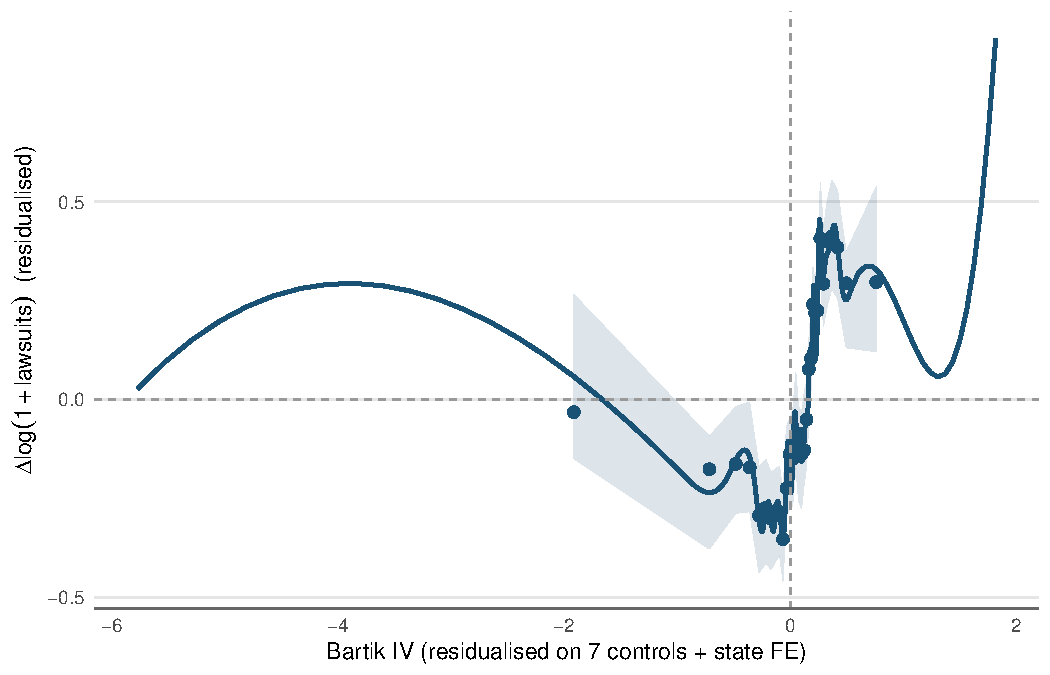
\includegraphics[width=0.88\textwidth,height=0.74\textheight,keepaspectratio]{../figures/binscatter_first_stage.pdf}
\end{center}
\end{frame}


% ============================================================
\section{Results: Electoral Competition}
% ============================================================

\begin{frame}{Electoral Competition --- Baseline Specification}
\footnotesize
\textit{Adversarial instrument (F\,=\,19.6). N\,=\,5,560, clusters\,=\,2,187. State FE\,$+$\,7 controls.}
\smallskip
\renewcommand{\arraystretch}{1.2}
\begin{tabular}{L{4.2cm}rrrcc}
  \toprule
  Outcome & Coef. & SE & $p$ & $t$ & tF reject? \\
  \midrule
  $\Delta$ Runner-up vote share  & $-$0.031 & 0.022 & 0.157 & $-$1.42 & \cross \\
  $\Delta$ Margin (W$-$RU)       & $+$0.062 & 0.043 & 0.151 & $+$1.44 & \cross \\
  $\Delta$ Winner vote share     & $+$0.031 & 0.025 & 0.213 & $+$1.25 & \cross \\
  $\Delta$ Winner majority (P50) & $+$0.140 & 0.090 & 0.122 & $+$1.55 & \cross \\
  $\Delta$ Log n candidates      & $-$0.066 & 0.039 & 0.092 & $-$1.69 & \cross \\
  \bottomrule
\end{tabular}
\normalsize
\medskip
\begin{columns}[T]
\begin{column}{0.50\textwidth}
\begin{block}{Directional pattern (winner consolidation)}
  \footnotesize
  All competition outcomes point toward winner consolidation: higher majority probability, wider margin, fewer candidates. Direction is consistent across all 6 specifications. \textbf{None survives tF correction} (tF$_\text{cv}$\,=\,2.18; max $|t|$\,=\,1.69).
\end{block}
\end{column}
\begin{column}{0.47\textwidth}
\begin{alertblock}{Candidate pool: marginal signal}
  \footnotesize
  Log candidates ($-$6.6\%, $p$\,=\,0.092) is the only outcome approaching conventional significance. Consistent with Besley \& Coate (1997): adversarial challenges raise the fixed cost of candidacy, deterring entry at the margin. Replicated in legislative analysis ($-$7.5\%, $p$\,=\,0.066).
\end{alertblock}
\end{column}
\end{columns}
\end{frame}


\begin{frame}{Electoral Competition --- Robustness Across Specifications}
\footnotesize
\textit{Outcome: $\Delta$ winner majority. All specifications, adversarial instrument.}
\smallskip
\renewcommand{\arraystretch}{1.2}
\begin{tabular}{L{4.2cm}rrrrc}
  \toprule
  Specification & Coef. & SE & $p$ & F & $N$ \\
  \midrule
  Baseline (state FE) & $+$0.140 & 0.090 & 0.122 & 19.6 & 5,560 \\
  Baseline, single-zone & $+$0.131 & 0.093 & 0.160 & 18.2 & 5,371 \\
  Full controls & $+$0.136 & 0.086 & 0.116 & 19.7 & 5,560 \\
  $\leq$200k voters & $+$0.128 & 0.091 & 0.161 & 19.3 & 5,338 \\
  Broader lawsuits control & $+$0.140 & 0.090 & 0.122 & 19.6 & 5,560 \\
  \bottomrule
\end{tabular}
\normalsize
\bigskip
\begin{itemize}
  \item Direction and magnitude are remarkably stable: coefficient ranges $+$0.128 to $+$0.140 across all specifications
  \item The result is not driven by control set, sample, or the non-adversarial baseline
  \item The precision gap (not reaching $p < 0.05$) is the fundamental limitation; a larger panel or stronger instrument would be needed to confirm
  \item \todo{Pre-period placebo (2016$\to$2020 outcomes): required to rule out pre-existing trend confounds}
\end{itemize}
\end{frame}


% ============================================================
\section{Results: Voter Behavior}
% ============================================================

\begin{frame}{Voter Behavior --- Baseline Specification}
\footnotesize
\textit{N\,=\,5,560, state FE\,$+$\,7 controls. Rates denominated on registered voters.}
\smallskip
\renewcommand{\arraystretch}{1.2}
\begin{tabular}{L{4.0cm}rrrcc}
  \toprule
  Outcome & Coef. & SE & $p$ & $t$ & tF reject? \\
  \midrule
  $\Delta$ Turnout rate      & $-$0.006 & 0.005 & 0.185 & $-$1.33 & \cross \\
  $\Delta$ Null vote rate    & $+$0.007 & 0.006 & 0.220 & $+$1.23 & \cross \\
  $\Delta$ Blank vote rate   & $+$\textbf{0.013} & \textbf{0.005} & \textbf{0.018} & $+$\textbf{2.36} & \tick \\
  $\Delta$ Valid vote rate   & $-$\textbf{0.026} & \textbf{0.013} & \textbf{0.038} & $-$\textbf{2.07} & \cross \\
  \bottomrule
\end{tabular}
\normalsize
\medskip
\begin{columns}[T]
\begin{column}{0.55\textwidth}
\begin{alertblock}{Main finding: blank vote rate}
  \footnotesize
  Adversarial judicialization $\uparrow$ by 1 SD ($\approx$ 0.16 units) $\Rightarrow$ blank rate $\uparrow$ by $0.013 \times 0.16 = 0.2$\,pp. At the mean blank rate of 1.9\%, this is a $\approx$10\% increase.\\[4pt]
  Effect survives tF correction ($|t|$\,=\,2.36\,$>$\,tF$_\text{cv}$\,=\,2.18). Valid-vote rate ($p$\,=\,0.038) is the accounting mirror and does \emph{not} survive tF. \textbf{Blank rate is the primary identified effect.}
\end{alertblock}
\end{column}
\begin{column}{0.43\textwidth}
\begin{block}{Precise nulls}
  \footnotesize
  Turnout ($p$\,=\,0.185) and null rate ($p$\,=\,0.220) are precise nulls. Adversarial judicial challenges do \emph{not} demobilize the electorate, contrary to negative advertising effects (Ansolabehere \& Iyengar 1995). The behavioral channel runs through expressive abstention, not non-participation.
\end{block}
\end{column}
\end{columns}
\end{frame}


\begin{frame}{Blank Vote Rate --- Interpretation}
\begin{columns}[T]
\begin{column}{0.55\textwidth}
\textbf{What blank votes signal:}\\
In Brazil, a blank vote (\emph{voto em branco}) is a deliberate choice to reject all listed candidates without spoiling the ballot. It requires specific action (pressing a button or writing `branco').
\bigskip

\textbf{Mechanism:}\\
Adversarial judicial challenges are publicly filed records that generate information about candidates' alleged conduct. Voters exposed to more diverse and intense judicial activity may face:
\begin{itemize}
  \item Increased uncertainty about all candidates' quality
  \item Negative updating about the entire political class (\emph{not} specific to a targeted candidate)
  \item Expressive dissatisfaction with the judicially-contested electoral environment
\end{itemize}
\bigskip
This is consistent with Lupia \& McCubbins (1998): institutional signals generate shortcuts, but in an adversarial environment they generate \emph{ambiguity} rather than clarity.
\end{column}
\begin{column}{0.43\textwidth}
\begin{block}{Literature anchor}
  \footnotesize
  Ferraz \& Finan (2008): publicly released audit information changes electoral outcomes in Brazil. Judicial filings are analogous: they are publicly available before election day and carry information about alleged wrongdoing.\\[4pt]
  \textbf{Key difference:} audits target specific corrupt incumbents (directional information); adversarial judicial waves are diffuse across all candidates (ambiguity-generating). This explains the blank vote outcome rather than an incumbent vote share effect.
\end{block}
\bigskip
\begin{block}{Robustness}
  \footnotesize
  Effect stable: coefficient 0.012--0.013 across baseline, single-zone, and full-controls specifications.
\end{block}
\end{column}
\end{columns}
\end{frame}


\begin{frame}{Open-Seat Heterogeneity --- Blank Vote Rate}
\begin{columns}[T]
\begin{column}{0.52\textwidth}
\textbf{Open seat} (46\% of municipalities, $N$\,=\,2,571):\\
2020 winner served two consecutive terms $\Rightarrow$ constitutionally term-limited in 2024. No incumbent on the ballot. Exogenous to 2024 litigation activity.
\bigskip

\textbf{Contested seat} (54\%, $N$\,=\,2,989):\\
2020 winner's first term. Incumbent can seek reelection. Voters have a focal candidate (support or oppose the incumbent).
\bigskip

\footnotesize
\renewcommand{\arraystretch}{1.3}
\begin{tabular}{L{2.2cm}rrrrc}
  \toprule
  Sample & Coef. & SE & $p$ & F & tF? \\
  \midrule
  All & $+$0.013 & 0.005 & 0.018 & 19.6 & \tick \\
  Open seat & $+$\textbf{0.030} & 0.014 & 0.028 & 10.6 & \cross$^{*}$ \\
  Contested & $+$0.003 & 0.005 & 0.546 & 15.3 & \cross \\
  \midrule
  \multicolumn{6}{l}{\scriptsize $^{*}$Conventional $p = 0.028$ but $|t| = 2.20 < \text{tF}_\text{cv} = 2.78$ (F\,=\,10.6).} \\
  \bottomrule
\end{tabular}
\normalsize
\end{column}
\begin{column}{0.46\textwidth}
\begin{alertblock}{Mechanism}
  \footnotesize
  The aggregate blank-rate effect runs almost entirely through \textbf{open-seat municipalities}.\\[4pt]
  \textbf{Why?} When no incumbent is running, voters lack a focal candidate. Adversarial judicial activity creates ambiguity about \emph{all} contenders simultaneously --- heightening the attractiveness of a blank vote.\\[4pt]
  When the incumbent runs, voters already have a valence benchmark (vote for or against the mayor). Legal noise is absorbed: the contested-seat effect is a structural zero.
\end{alertblock}
\medskip
\begin{block}{Caveat: weakened instrument}
  \footnotesize
  Open-seat subgroup: F\,=\,10.6 (vs.\,19.6 full sample). Smaller municipalities likely to have longer-serving incumbents but also less electoral litigation variation. The tF correction is therefore stricter (tF$_\text{cv}$\,=\,2.78); effect survives conventional but not weak-IV-robust inference.
\end{block}
\end{column}
\end{columns}
\end{frame}


\begin{frame}{Voter Behavior --- Forest Plot (All Specs)}
\begin{center}
  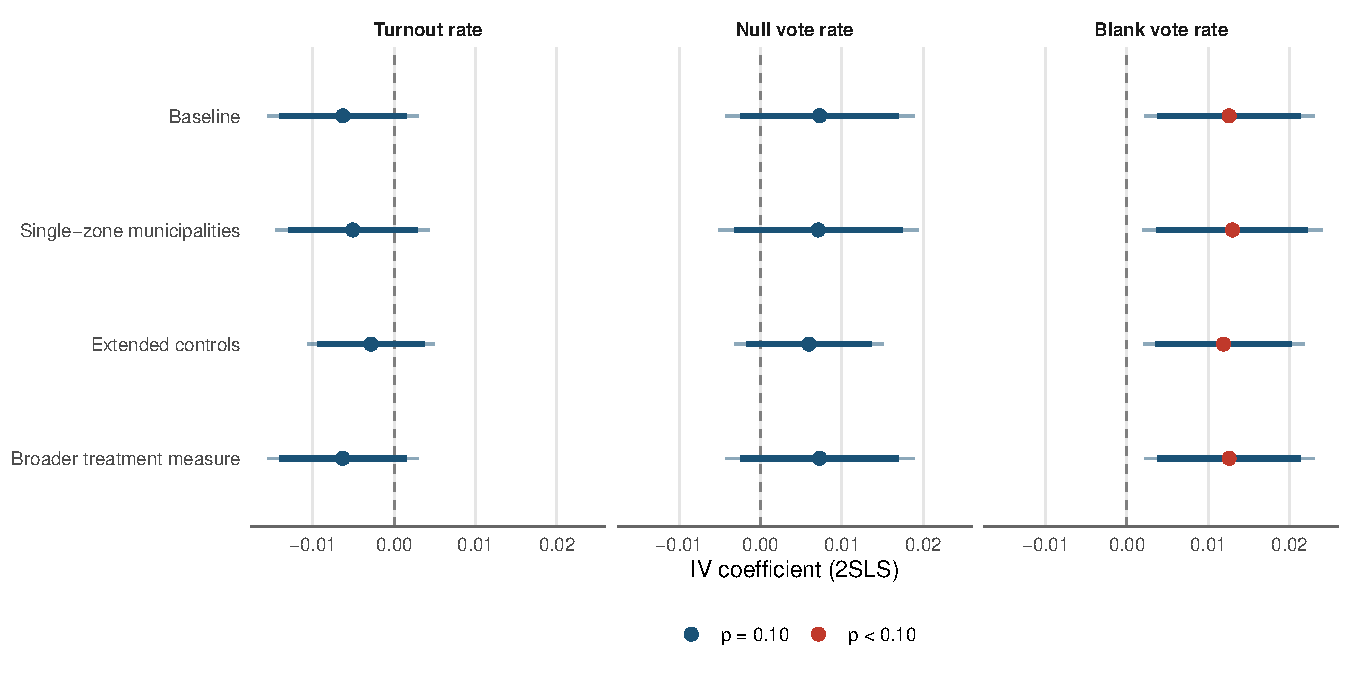
\includegraphics[width=\textwidth,height=0.76\textheight,keepaspectratio]{../figures/forest_voter_behavior.pdf}
\end{center}
\end{frame}


% ============================================================
\section{Results: Composition}
% ============================================================

\begin{frame}{Candidate Pool and Composition --- Baseline}
\footnotesize
\textit{Adversarial instrument, baseline specification. N\,=\,5,560, clusters\,=\,2,187.}
\smallskip
\renewcommand{\arraystretch}{1.2}
\begin{tabular}{L{4.5cm}rrrc}
  \toprule
  Outcome & Coef. & SE & $p$ & tF reject? \\
  \midrule
  $\Delta$ Log n candidates (exec.)    & $-$0.066 & 0.039 & 0.092 & \cross \\
  $\Delta$ New-cand.\ vote share (exec.)& $-$0.010 & 0.050 & 0.848 & \\
  $\Delta$ Incumbent vote share (exec.) & $+$0.010 & 0.049 & 0.844 & \\[3pt]
  $\Delta$ Female vote share            & $-$0.093 & 0.048 & 0.052 & \cross \\
  $\Delta$ Winner is female             & $-$0.123 & 0.063 & 0.052 & \cross \\
  $\Delta$ Winner is new entrant        & $-$0.002 & 0.073 & 0.982 & \\
  \bottomrule
\end{tabular}
\normalsize
\medskip
\begin{columns}[T]
\begin{column}{0.50\textwidth}
\begin{block}{Entry deterrence (not composition shift)}
  \footnotesize
  The candidate count reduction ($-$6.6\%) is directional, not significant. But it replicates across executive and legislative arenas (next slide), lending it more credibility. New-entrant and incumbent vote shares are both near zero --- the field shrinks, but without systematic reallocation toward any type.
\end{block}
\end{column}
\begin{column}{0.47\textwidth}
\begin{alertblock}{Gender: directional, not robust}
  \footnotesize
  Female vote share ($-$9.3\,pp, $p$\,=\,0.052) and female winner probability ($-$12.3\,pp, $p$\,=\,0.052) are just below 5\% but do not survive tF correction ($|t|$\,=\,1.94 and 1.94\,$<$\,2.18). Direction is suggestive --- adversarial legal challenges may disadvantage women candidates --- but requires richer candidate-level data to confirm.
\end{alertblock}
\end{column}
\end{columns}
\end{frame}


\begin{frame}{Candidate Entrant Typology --- New Variables}
\begin{columns}[T]
\begin{column}{0.52\textwidth}
\textbf{Three entrant types, 4 electoral cycles (2012--2024):}
\footnotesize
\begin{itemize}
  \item \textbf{Pure new entrant:} no prior mayoral candidacy anywhere in 2012, 2016, or 2020 ($\bar{s}_{2024}$\,=\,55\%)
  \item \textbf{Serial challenger:} ran in the same municipality in 2020, lost, running again ($\bar{s}_{2024}$\,=\,13\%)
  \item \textbf{Cross-cycle returner:} has prior history but sat out 2020 entirely; returning after a cycle gap ($\bar{s}_{2024}$\,=\,9\%)
\end{itemize}
\normalsize
\bigskip
\textbf{Question:} Does adversarial judicialization reshape \emph{who enters}, not just \emph{how many}?
\end{column}
\begin{column}{0.46\textwidth}
\begin{block}{IV Results: Entry Composition}
  \footnotesize
  \renewcommand{\arraystretch}{1.2}
  \begin{tabular}{L{2.8cm}rrr}
    \toprule
    Outcome & Coef. & SE & $p$ \\
    \midrule
    $\Delta$ New entrant share & $-$0.011 & 0.043 & 0.793 \\
    $\Delta$ Serial challenger & $+$0.007 & 0.026 & 0.802 \\
    $\Delta$ Cross-cycle ret. & $+$0.005 & 0.025 & 0.861 \\
    \midrule
    \multicolumn{4}{l}{\scriptsize Baseline spec. N\,=\,5,560, F\,=\,19.6.} \\
    \bottomrule
  \end{tabular}
\end{block}
\medskip
\begin{alertblock}{Interpretation}
  \footnotesize
  All three entrant-type shares are precise nulls. Judicialization does not \emph{selectively screen} entrant types --- it reduces the count ($-$6.6\%) without reshaping the pool's experience composition.\\[4pt]
  Entry deterrence is a \textbf{quantity} effect, not a \textbf{selection} effect.
\end{alertblock}
\end{column}
\end{columns}
\end{frame}


% ============================================================
\section{Results: Legislative}
% ============================================================

\begin{frame}{Legislative Analysis --- City Council Elections (Vereadores)}
\begin{columns}[T]
\begin{column}{0.55\textwidth}
\textbf{Same instrument, different electoral arena:}
\begin{itemize}
  \item Brazil's city councils (\emph{Câmaras Municipais}) elect 9--55 \emph{vereadores} depending on population (CF Art.~29-IV)
  \item Pre-election challenges also target legislative candidates
  \item \textbf{Multi-seat proportional} system --- different from the plurality mayoral race
\end{itemize}
\bigskip
\textbf{Identification:} same municipality-level Bartik IV (F\,$\approx$\,19.4). The shift in adversarial litigation waves applies to the same municipality and electoral environment. Endogenous: $\Delta\log(1+\text{competition lawsuits})$ at municipality level (same treatment).
\end{column}
\begin{column}{0.43\textwidth}
\begin{block}{Outcome Families}
  \footnotesize
  \textbf{Candidate pool:}
  \begin{itemize}
    \item Total candidates, female/nonwhite shares
    \item New candidates, incumbents, party count
  \end{itemize}
  \textbf{Elected composition:}
  \begin{itemize}
    \item Elected female/nonwhite shares
    \item Higher-education share, mean age
    \item Incumbent reelected share
  \end{itemize}
  \textbf{Party competition:}
  \begin{itemize}
    \item Party count, coalition count
  \end{itemize}
\end{block}
\medskip
\begin{block}{Instrument}
\footnotesize N\,=\,5,560; clusters\,=\,2,187; F\,=\,19.4.
\end{block}
\end{column}
\end{columns}
\end{frame}


\begin{frame}{Legislative IV Results}
\footnotesize
\textit{Baseline specification. N\,=\,5,560, clusters\,=\,2,187. State FE\,$+$\,7 controls. F\,=\,19.4.}
\smallskip
\renewcommand{\arraystretch}{1.2}
\begin{tabular}{L{5.2cm}rrrr}
  \toprule
  Outcome & Coef. & SE & $p$ & Sig. \\
  \midrule
  \multicolumn{5}{l}{\textit{Candidate pool}} \\
  $\Delta$ Log total candidates        & $-$0.075 & 0.041 & 0.066 & $\dagger$ \\
  $\Delta$ Female candidate share      & $-$0.006 & 0.006 & 0.370 & \\
  $\Delta$ Nonwhite candidate share    & $-$0.018 & 0.019 & 0.346 & \\
  $\Delta$ New candidate share         & $-$0.020 & 0.016 & 0.217 & \\
  $\Delta$ Eff.\ party count (candidates) & $-$0.264 & 0.301 & 0.381 & \\[3pt]
  \multicolumn{5}{l}{\textit{Elected composition}} \\
  $\Delta$ Elected female share        & $+$0.013 & 0.022 & 0.554 & \\
  $\Delta$ Elected nonwhite share      & $-$0.027 & 0.026 & 0.288 & \\
  $\Delta$ Incumbent reelected share   & $+$0.006 & 0.025 & 0.797 & \\[3pt]
  \multicolumn{5}{l}{\textit{Party competition}} \\
  $\Delta$ Party count                 & $-$0.260 & 0.354 & 0.463 & \\
  $\Delta$ Coalition count             & $+$0.074 & 0.066 & 0.266 & \\
  \midrule
  \multicolumn{5}{l}{\footnotesize $\dagger p < 0.10$. SE clustered by principal electoral zone.} \\
  \bottomrule
\end{tabular}
\normalsize
\end{frame}


\begin{frame}{Executive vs.\ Legislative: Comparing Effects}
\begin{columns}[T]
\begin{column}{0.55\textwidth}
\textbf{Same instrument (F\,$\approx$\,19--20), two electoral arenas:}
\bigskip
\renewcommand{\arraystretch}{1.3}
\footnotesize
\begin{tabular}{L{3.4cm}cc}
  \toprule
  Outcome & Executive & Legislative \\
  \midrule
  $\Delta$ Log candidates & $-$0.066$^\dagger$ & $-$0.075$^\dagger$ \\
  Winner consolidation & directional & --- \\
  Female share & $-$0.093$^\dagger$ & $-$0.006 \\
  Blank rate & $+$0.013$^{**}$ & --- \\
  Elected composition & null & null \\
  Party competition & null & null \\
  \bottomrule
  \multicolumn{3}{l}{\scriptsize $^{**}p<0.05$ (tF corrected); $^\dagger p < 0.10$ (uncorrected).}
\end{tabular}
\normalsize
\end{column}
\begin{column}{0.43\textwidth}
\begin{block}{Interpretation}
  \footnotesize
  \textbf{Both arenas:} candidate pool contracts ($-$7\%) consistently --- entry deterrence channel is the most robust structural finding. Consistent with Besley \& Coate (1997).\\[4pt]
  \textbf{Executive only:} winner consolidation (directional), blank rate (significant), gender effects (borderline) --- these run through competition dynamics specific to the single-winner plurality race.\\[4pt]
  \textbf{Legislative:} multi-seat proportional allocation dampens the competitive displacement effects visible in executive races. No effect on who wins seats or on party composition.
\end{block}
\end{column}
\end{columns}
\end{frame}


% ============================================================
\section{Mechanism: Family-Split IV}
% ============================================================

\begin{frame}{Family-Split IV --- Mechanism Analysis}
\begin{columns}[T]
\begin{column}{0.55\textwidth}
\textbf{Motivation:}\\
The aggregate Bartik IV combines topics from four litigation families. Do different \emph{types} of adversarial challenges operate through different mechanisms?
\bigskip

\textbf{Approach (AMV 2025, Section 6):}\\
Construct a \emph{family-specific} Bartik IV for each topic family:
\[
Z_m^{f} = \sum_{k \in f} s_{m,k,2020} \cdot g_{\text{UF},k,-m}
\]
Each $Z_m^f$ instruments the \emph{family-specific} endogenous: $\Delta\log(1+\ell_{m,f})$. This identifies a family-level LATE --- different from the aggregate.
\end{column}
\begin{column}{0.43\textwidth}
\begin{block}{Four Litigation Families}
  \footnotesize
  \renewcommand{\arraystretch}{1.2}
  \begin{tabular}{lrrc}
    \toprule
    Family & F & N & Identified? \\
    \midrule
    Campaign conduct & 36.0 & 3,937 & \tick \\
    Information env. & 19.7 & 3,861 & \tick \\
    Abuse of office & 7.8 & 3,311 & \cross \\
    Eligibility/Ballot & 8.4 & 1,772 & \cross \\
    \bottomrule
  \end{tabular}
  \normalsize
\end{block}
\medskip
\footnotesize
\textbf{Campaign conduct:} campaign propaganda, prohibited conduct, vote-buying\\[4pt]
\textbf{Information environment:} media, internet propaganda, right of reply\\[4pt]
\textbf{Eligibility/Ballot access:} registration challenges, impugna\c{c}\~{a}o\\[4pt]
\textbf{Abuse of office:} economic and political power abuses
\end{column}
\end{columns}
\end{frame}


\begin{frame}{Family IV Results --- Primary Outcomes}
\footnotesize
\textit{Family-specific Bartik IV instruments family-specific endogenous. Baseline state FE + 7 controls.}
\smallskip
\renewcommand{\arraystretch}{1.2}
\begin{tabular}{L{2.6cm}rrrrrr}
  \toprule
  & \multicolumn{2}{c}{$\Delta$ Runner-up} & \multicolumn{2}{c}{$\Delta$ Margin} & \multicolumn{2}{c}{$\Delta$ Log cand.} \\
  \cmidrule(lr){2-3}\cmidrule(lr){4-5}\cmidrule(lr){6-7}
  Family (F$^{fs}$) & Coef. & $p$ & Coef. & $p$ & Coef. & $p$ \\
  \midrule
  Campaign (F\,=\,36) & $-$0.007 & 0.545 & $+$0.018 & 0.442 & $-$0.004 & 0.836 \\
  Info.\ env.\ (F\,=\,20) & $-$0.010 & 0.511 & $+$0.034 & 0.250 & $+$0.013 & 0.665 \\
  \midrule
  \multicolumn{7}{l}{\footnotesize Abuse of office (F\,=\,7.8) and eligibility (F\,=\,8.4): weak instrument --- estimates unreliable.} \\
  \bottomrule
\end{tabular}
\normalsize
\medskip
\begin{columns}[T]
\begin{column}{0.55\textwidth}
\begin{block}{Null across well-identified families}
  \footnotesize
  Both campaign-conduct and information-environment sub-instruments produce null effects across all competition outcomes. This is consistent with the aggregate null --- the aggregate result is not concealing strong but cancelling effects across family types. Direction is non-systematic (not all positive or all negative), further supporting the null.
\end{block}
\end{column}
\begin{column}{0.43\textwidth}
\begin{alertblock}{Implications}
  \footnotesize
  The blank-rate effect and the candidate-pool reduction are not attributable to a single mechanism family with the currently available family instruments. Both campaign conduct and information environment challenges contribute to the aggregate treatment without producing detectable competition effects through their separate channels.
\end{alertblock}
\end{column}
\end{columns}
\end{frame}


% ============================================================
\section{Robustness}
% ============================================================

\begin{frame}{Robustness: Population Subsamples}
\begin{columns}[T]
\begin{column}{0.55\textwidth}
\textbf{Art.~29-II CF/88:} municipalities with $>$200,000 registered voters hold a mandatory second round if no candidate wins $>$50\%
\bigskip

\textbf{Two subsamples:}
\begin{itemize}
  \item $\leq$200k voters: 5,338 --- strictly single-round; homogeneous institutional regime
  \item $>$200k voters: 222 --- conditional second round; instrument loses power (F\,$<$\,1)
\end{itemize}
\bigskip
\textbf{Large-city failure:} consistent with instrument design --- larger municipalities tend to dominate their state shifts, so the LOO construction leaves less identifying variation.
\end{column}
\begin{column}{0.43\textwidth}
\begin{block}{$\Delta$ Winner majority by subsample}
  \footnotesize
  \renewcommand{\arraystretch}{1.2}
  \begin{tabular}{lrrrr}
    \toprule
    Sample & Coef. & SE & $p$ & F \\
    \midrule
    All ($N$\,=\,5,560) & $+$0.140 & 0.090 & 0.122 & 19.6 \\
    $\leq$200k ($N$\,=\,5,338) & $+$0.128 & 0.091 & 0.161 & 19.3 \\
    $>$200k ($N$\,=\,222) & n.a. & & & $<$1 \\
    \bottomrule
  \end{tabular}
\end{block}
\bigskip
\begin{block}{Single-zone municipalities}
  \footnotesize
  N\,=\,5,371 (96.6\%): municipality = zone = cluster; exact correspondence. Coefficients essentially identical to full sample; F\,=\,18.2.
\end{block}
\end{column}
\end{columns}
\end{frame}


\begin{frame}{Robustness: Extended Controls and Broader Lawsuits}
\begin{columns}[T]
\begin{column}{0.55\textwidth}
\textbf{14-variable extended control set:}\\
Adds ENP 2016, candidate composition (gender, ethnicity, education), party/coalition count, voter behavior baseline, candidate experience.
\bigskip

\textbf{Caveat:} some extended controls are outcome-adjacent (2020 candidate composition may reflect prior judicialization). Use as sensitivity only.
\bigskip

\textbf{Broader lawsuits control:}\\
Adds $\log(1 + \ell_m^{\text{no-RRC}})$ in 2020 as a covariate --- the broader competition lawsuit stock (excluding only RRC). Tests whether the adversarial IV effect is distinct from general pre-existing litigation activity.
\end{column}
\begin{column}{0.43\textwidth}
\begin{block}{Blank rate across control sets}
  \footnotesize
  \renewcommand{\arraystretch}{1.2}
  \begin{tabular}{lrrrr}
    \toprule
    Spec & Coef. & SE & $p$ & F \\
    \midrule
    7 baseline & $+$0.013 & 0.005 & 0.018 & 19.6 \\
    14 extended & $+$0.012 & 0.005 & 0.022 & 19.7 \\
    Broader ctrl & $+$0.013 & 0.005 & 0.018 & 19.6 \\
    \midrule
    Margin (7 base.) & $+$0.062 & 0.043 & 0.151 & 19.6 \\
    Margin (14 ext.) & $+$0.057 & 0.042 & 0.180 & 19.7 \\
    Margin (broader) & $+$0.062 & 0.043 & 0.151 & 19.6 \\
    \bottomrule
  \end{tabular}
\end{block}
\footnotesize\textit{Blank rate result is stable to control set and to conditioning on broader lawsuit baseline.}
\end{column}
\end{columns}
\end{frame}


% ============================================================
\section{Conclusion}
% ============================================================

\begin{frame}{Summary of Findings}
\begin{columns}[T]
\begin{column}{0.57\textwidth}
\begin{enumerate}
  \item \textbf{Blank vote rate --- main finding:}\\
  $+$1.3\,pp ($p$\,=\,0.018; survives tF correction). Adversarial judicialization generates voter ambivalence, expressed through deliberate blank votes. Turnout and null rate: precise nulls. No demobilization.
  \bigskip
  \item \textbf{Candidate pool contraction (marginal):}\\
  $-$6.6\% executive ($p$\,=\,0.092); $-$7.5\% legislative ($p$\,=\,0.066). Consistent across arenas --- entry deterrence is the most robust structural channel.
  \bigskip
  \item \textbf{Winner consolidation (directional):}\\
  All competition outcomes favor the winner: higher majority, wider margin. Direction stable across all 5 core specifications. Not statistically identified after tF correction.
  \bigskip
  \item \textbf{Open-seat heterogeneity:}\\
  Blank rate effect concentrated in open seats ($+$3.0\,pp, $p$\,=\,0.028) vs.\ contested-seat structural zero ($+$0.3\,pp, $p$\,=\,0.55). Mechanism: no focal incumbent $\Rightarrow$ judicial ambiguity translates directly into blank votes.
  \bigskip
  \item \textbf{Entry is a quantity effect, not a selection effect:}\\
  Entrant composition (new, serial, returning) does not change. Judicialization reduces the pool without reshaping who enters.
  \bigskip
  \item \textbf{Legislative and family splits:} precise nulls on composition; no single litigation family drives results.
\end{enumerate}
\end{column}
\begin{column}{0.41\textwidth}
\begin{alertblock}{Main Takeaway}
  Credibly identified estimates from a Bartik shift-share IV (F\,=\,19.6, tF-corrected inference).
  \medskip\\
  The primary causal effect of adversarial judicialization on Brazilian municipal elections is voter ambivalence --- a significant rise in blank votes --- rather than competitive displacement or mobilization.
  \medskip\\
  Entry deterrence is the most consistent structural finding across arenas. Winner consolidation is the most economically plausible pattern; it remains statistically underpowered.
\end{alertblock}
\end{column}
\end{columns}
\end{frame}


\begin{frame}{Contributions, Open Questions, and Next Steps}
\begin{columns}[T]
\begin{column}{0.55\textwidth}
\textbf{Contributions:}
\begin{itemize}
  \item First Bartik IV applied to electoral judicialization; blueprint for causal identification of litigation effects in political economy
  \item Full GPS/BHJ/AKM compliance; tF correction applied
  \item Systematic administrative-vs-adversarial distinction: a measurement contribution to the electoral law literature
  \item Cross-arena comparison (executive vs.\ legislative): entry deterrence replicates; competition effects arena-specific
\end{itemize}
\medskip
\textbf{Open questions requiring new data:}
\begin{itemize}
  \item \todo{Pre-period placebo: 2016$\to$2020 outcomes as falsification test}
  \item \todo{Case outcomes (win/loss rulings) as second instrument}
  \item \todo{TRE judge composition heterogeneity}
  \item \todo{Longer panel: 2012--2024 for trend identification}
\end{itemize}
\end{column}
\begin{column}{0.43\textwidth}
\begin{block}{Pending analysis}
  \begin{itemize}
    \item Romano--Wolf multiple testing correction across outcome families
    \item Concavity analysis: zero-share vs.\ positive-share municipalities (intensive vs.\ extensive margin)
    \item \tick~Open-seat heterogeneity: done (blank rate 3$\times$ larger in open seats)
    \item \tick~Entry typology: done (quantity effect, not selection)
    \item Female candidate heterogeneity: candidate-level analysis of gender differential exposure
  \end{itemize}
\end{block}
\begin{block}{Literature Connections}
  \footnotesize
  GPS (2020); BHJ (2022); AKM (2019); Lee et al.\ (2022); Ash, Morelli \& Vannoni (2025); Ferraz \& Finan (2008); Besley \& Coate (1997); Helmke \& Staton (2011)
\end{block}
\end{column}
\end{columns}
\end{frame}


% ============================================================
% APPENDIX
% ============================================================
\appendix

\begin{frame}[allowframebreaks]{Appendix A: Full First-Stage Table}
\footnotesize
\textbf{Adversarial instrument (\texttt{bartik\_iv\_2020\_2024}). Single specification.}\\[4pt]
Adversarial filter applied at data construction stage (class and subject-code exclusions from TSE taxonomy; mandatory administrative filings excluded). One instrument, one endogenous variable.
\medskip
\renewcommand{\arraystretch}{1.3}
\begin{tabular}{L{4.2cm}rrrrcr}
  \toprule
  Specification & Coef. & SE & $t$ & F-stat & tF$_\text{cv}$ & $N$ \\
  \midrule
  Baseline (state FE) & 1.791 & 0.405 & 4.43 & \textbf{19.6} & 2.18 & 5,560 \\
  Baseline, single-zone & 1.801 & 0.422 & 4.27 & \textbf{18.2} & 2.23 & 5,371 \\
  Full controls & 1.799 & 0.406 & 4.44 & \textbf{19.7} & 2.18 & 5,560 \\
  $\leq$200k voters & 1.869 & 0.426 & 4.39 & \textbf{19.3} & 2.19 & 5,338 \\
  Broader lawsuits ctrl & 1.792 & 0.405 & 4.43 & \textbf{19.6} & 2.18 & 5,560 \\
  Topic shares ctrl$^{*}$ & $-$0.656 & 0.926 & $-$0.71 & \textbf{0.5} & --- & 2,824 \\
  \midrule
  \multicolumn{7}{l}{\footnotesize SE clustered by principal electoral zone. F\,=\,$(t$-stat)$^2$.} \\
  \multicolumn{7}{l}{\footnotesize tF$_\text{cv}$: weak-IV-robust critical value (Lee et al.\ 2022, Table 1), 5\% level.} \\
  \multicolumn{7}{l}{\footnotesize $^{*}$Identification collapses: the 2020 shares ARE the instrument's variation.} \\
  \bottomrule
\end{tabular}
\normalsize
\end{frame}


\begin{frame}[allowframebreaks]{Appendix B: Full IV Table --- Competition and Voter Behavior}
\footnotesize
\renewcommand{\arraystretch}{1.2}
\textbf{Adversarial instrument. Baseline specification. N\,=\,5,560, clusters\,=\,2,187.}
\smallskip
\begin{tabular}{L{4.2cm}rrrrr}
  \toprule
  Outcome & Coef. & SE & $t$ & $p$ & tF$^*$? \\
  \midrule
  \multicolumn{6}{l}{\textit{Competition}} \\
  $\Delta$ Runner-up & $-$0.031 & 0.022 & $-$1.42 & 0.157 & \cross \\
  $\Delta$ Margin & $+$0.062 & 0.043 & $+$1.44 & 0.151 & \cross \\
  $\Delta$ Winner vote & $+$0.031 & 0.025 & $+$1.25 & 0.213 & \cross \\
  $\Delta$ Majority & $+$0.140 & 0.090 & $+$1.55 & 0.122 & \cross \\
  $\Delta$ Log candidates & $-$0.066 & 0.039 & $-$1.69 & 0.092 & \cross \\[3pt]
  \multicolumn{6}{l}{\textit{Voter behavior}} \\
  $\Delta$ Turnout rate & $-$0.006 & 0.005 & $-$1.33 & 0.185 & \cross \\
  $\Delta$ Null rate & $+$0.007 & 0.006 & $+$1.23 & 0.220 & \cross \\
  $\Delta$ Blank rate & $+$\textbf{0.013} & \textbf{0.005} & $+$\textbf{2.36} & \textbf{0.018} & \tick \\
  $\Delta$ Valid vote rate & $-$0.026 & 0.013 & $-$2.07 & 0.038 & \cross \\
  \midrule
  \multicolumn{6}{l}{\footnotesize $^{*}$tF$_\text{cv}$\,=\,2.18 (F\,=\,19.6); \tick\,=\,$|t| > 2.18$. SE clustered by principal electoral zone.} \\
  \bottomrule
\end{tabular}
\normalsize
\end{frame}


\begin{frame}[allowframebreaks]{Appendix C: Full IV Table --- Composition}
\footnotesize
\renewcommand{\arraystretch}{1.2}
\textbf{Adversarial instrument. Baseline state FE. N\,=\,5,560.}
\smallskip
\begin{tabular}{L{4.5cm}rrrr}
  \toprule
  Outcome & Coef. & SE & $t$ & $p$ \\
  \midrule
  $\Delta$ Female vote share & $-$0.093 & 0.048 & $-$1.94 & 0.052 \\
  $\Delta$ Nonwhite vote share & $-$0.039 & 0.042 & $-$0.94 & 0.348 \\
  $\Delta$ New cand.\ vote share & $-$0.010 & 0.050 & $-$0.19 & 0.848 \\
  $\Delta$ Incumbent vote share & $+$0.010 & 0.049 & $+$0.20 & 0.844 \\
  $\Delta$ Winner is female & $-$0.123 & 0.063 & $-$1.94 & 0.052 \\
  $\Delta$ Winner is new entrant & $-$0.002 & 0.073 & $-$0.02 & 0.982 \\
  $\Delta$ Winner ideology & $-$0.168 & 0.205 & $-$0.82 & 0.412 \\
  Pedersen volatility & $-$0.010 & 0.038 & $-$0.25 & 0.801 \\
  \midrule
  \multicolumn{5}{l}{\footnotesize SE clustered by principal electoral zone. tF$_\text{cv}$\,=\,2.18; no composition outcome survives tF correction.} \\
  \bottomrule
\end{tabular}
\normalsize
\end{frame}


\begin{frame}{Appendix D: Case Classification}
\begin{columns}[T]
\begin{column}{0.55\textwidth}
\textbf{Competition-relevant adversarial case criteria:}
\begin{enumerate}
  \item Mayoral candidate (\emph{prefeito}) is the respondent
  \item Filed before election day
  \item Case class and subject are not on the administrative exclusion list
\end{enumerate}
\bigskip
\textbf{Examples of included subjects:}\\
\footnotesize
Abuso do Poder Econ\^{o}mico, Abuso do Poder Pol\'{i}tico, Capta\c{c}\~{a}o Il\'{i}cita de Sufr\'{a}gio, Propagan\-da Elei\-to\-ral Ir\-re\-gu\-lar, Con\-du\-ta Ve\-da\-da a Agen\-te P\'{u}b\-li\-co, Uso In\-de\-vi\-do dos Meios de Co\-mu\-nica\-\c{c}\~{a}o, Im\-pug\-na\-\c{c}\~{a}o de Re\-gis\-tro de Can\-di\-da\-tu\-ra, Fal\-si\-fi\-ca\-\c{c}\~{a}o de Do\-cu\-men\-to
\end{column}
\begin{column}{0.43\textwidth}
\begin{block}{Case Volume (2020 / 2024)}
  \footnotesize
\renewcommand{\arraystretch}{1.2}
\begin{tabular}{lrr}
  \toprule
  Category & 2020 & 2024 \\
  \midrule
  Mandatory registration (RRC) & $\sim$994k & $\sim$841k \\
  Coalition registration (DRAP) & $\sim$137k & $\sim$118k \\
  Adversarial competition cases & $\sim$385k & $\sim$340k \\
  \bottomrule
\end{tabular}
\end{block}
\medskip
\begin{alertblock}{Filter logic}
\footnotesize The adversarial filter excludes entire administrative \emph{classes} (mandatory processing) as well as specific \emph{subjects} that are procedurally rather than substantively adversarial. This is stricter than simply removing RRC and DRAP topic entries.
\end{alertblock}
\end{column}
\end{columns}
\end{frame}


\begin{frame}{Appendix E: Instrument Distribution, Geography, and Visual IV}
\begin{columns}[T]
\begin{column}{0.42\textwidth}
  \textbf{Figure E1: Distribution of Bartik IV}\\
  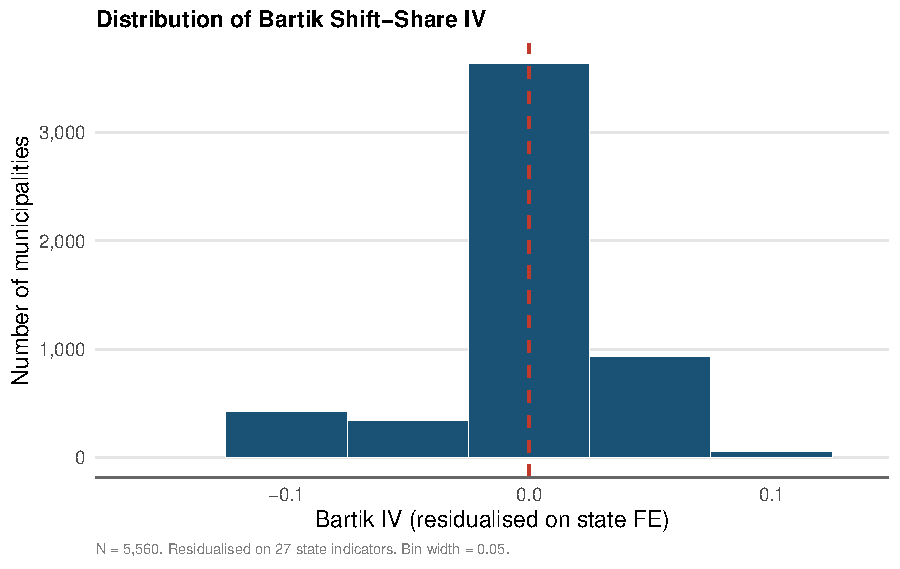
\includegraphics[width=\textwidth,height=0.60\textheight,keepaspectratio]{../figures/bartik_histogram.pdf}
\end{column}
\begin{column}{0.56\textwidth}
  \textbf{Figure E2: Geographic distribution}\\
  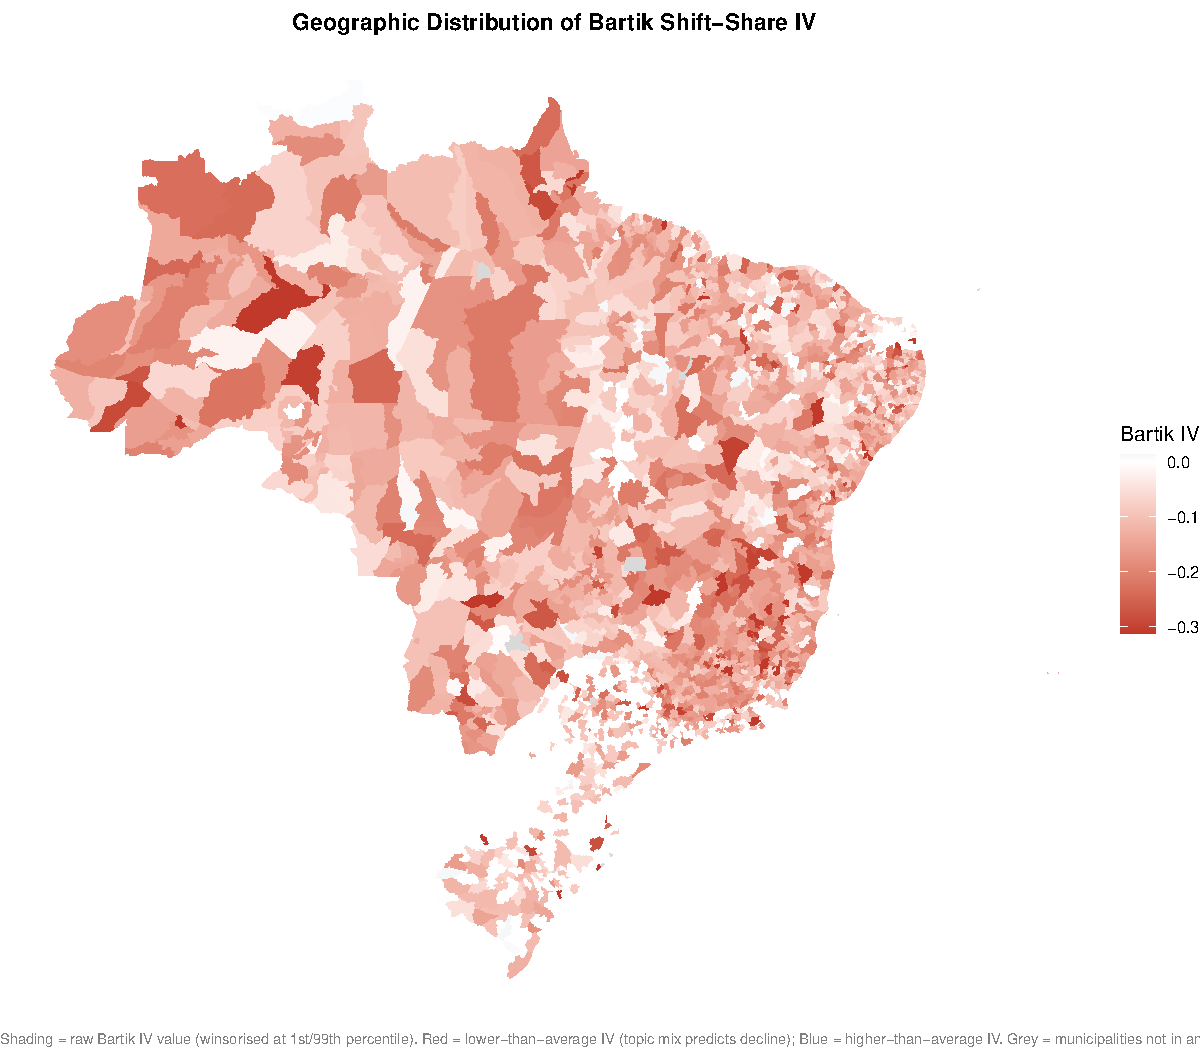
\includegraphics[width=\textwidth,height=0.60\textheight,keepaspectratio]{../figures/bartik_choropleth.pdf}
\end{column}
\end{columns}
\medskip
\footnotesize\textit{IV residualized on state FE for histogram. Map: raw Bartik IV by municipality (grey = not in sample). Visual IV graph ($\tau_k$ vs.\ $F_k$, sized by $|\alpha_k|$): see \texttt{output/figures/visual\_iv\_grid.pdf}.}
\end{frame}


\begin{frame}[allowframebreaks]{Appendix F: Balance Table}
\footnotesize
\renewcommand{\arraystretch}{1.2}
\textbf{Adversarial instrument regressed on each covariate. State FE, SE clustered by zone.}
\smallskip
\begin{tabular}{L{5cm}rrr}
  \toprule
  Covariate & Coef. & SE & $p$ \\
  \midrule
  Log population (2010) & $-0.543$ & $0.256$ & $0.034$ \\
  Urban share (2010) & $-0.024$ & $0.028$ & $0.385$ \\
  Log income per capita (2010) & $+0.164$ & $0.049$ & $0.001$ \\
  Margin 2016 & $+0.089$ & $0.041$ & $0.030$ \\
  ENP 2016 & $-0.256$ & $0.142$ & $0.072$ \\
  Turnout rate 2020 & $+0.040$ & $0.012$ & $0.001$ \\
  Female candidate share 2020 & $-0.075$ & $0.046$ & $0.101$ \\
  Nonwhite candidate share 2020 & $-0.050$ & $0.067$ & $0.458$ \\
  Log n candidates 2020 & $-0.127$ & $0.084$ & $0.129$ \\
  \midrule
  \multicolumn{4}{l}{\footnotesize 3 of 9 covariates $p < 0.05$. Correlations reflect that larger, richer,} \\
  \multicolumn{4}{l}{\footnotesize higher-turnout municipalities had more diverse 2020 litigation portfolios.} \\
  \multicolumn{4}{l}{\footnotesize \textbf{All three pre-determined controls included in every specification.}} \\
  \bottomrule
\end{tabular}
\normalsize
\medskip
\textbf{Interpretation:} Non-random share exposure is expected when municipalities differ systematically. The identification claim is that these differences are absorbed by the pre-determined controls and state FE. The GPS balance tests (gps\_balance\_tests.csv) run more detailed regressions per top topic.
\end{frame}


\begin{frame}{Appendix G: Family IV --- First Stage by Family}
\footnotesize
\textit{Each family IV instruments its family-specific endogenous ($\Delta\log(1+\ell_{m,f})$). Baseline spec.}
\smallskip
\renewcommand{\arraystretch}{1.2}
\begin{tabular}{L{3.5cm}rrrrc}
  \toprule
  Family & Endog.\ coef. & SE & F & $N$ & Identified? \\
  \midrule
  Campaign conduct & $+$1.61 & 0.27 & 36.0 & 3,937 & \tick \\
  Information env. & $+$2.29 & 0.52 & 19.7 & 3,861 & \tick \\
  Abuse of office & $-$2.54 & 0.91 & 7.8 & 3,311 & \cross \\
  Eligibility/Ballot & $-$0.20 & 0.07 & 8.4 & 1,772 & \cross \\
  \bottomrule
\end{tabular}
\normalsize
\medskip
\footnotesize
\textbf{Notes:} N varies by family because family-IV is defined only for municipalities with nonzero family exposure ($s_{mk,2020} > 0$ for topic $k$ in family $f$). Negative coefficients for abuse and eligibility families indicate the Bartik IV for those families is negatively associated with own-family lawsuit growth --- consistent with diffuse spillover dynamics. These families should not be interpreted.\\[4pt]
\textbf{Abuse of office} and \textbf{eligibility/ballot} families have F $<$ 10; weak-instrument concerns preclude reliable 2SLS inference. \textbf{Campaign conduct} (F\,=\,36) and \textbf{information environment} (F\,=\,20) are the identified families.
\end{frame}


\begin{frame}[fragile]{Appendix H: R Estimation Code (fixest)}
\begin{columns}[T]
\begin{column}{0.55\textwidth}
All main results estimated in \textbf{R} using \texttt{fixest::feols()} v0.14.1:
\bigskip

\textbf{IV formula (adversarial instrument):}
\begin{small}
\begin{verbatim}
feols(outcome ~ controls | SG_UF |
  delta_log1p_competition_lawsuits
    ~ bartik_iv_2020_2024,
  data, cluster = ~cluster_id)
\end{verbatim}
\end{small}
\bigskip

\textbf{LIML (confirmation only):}
\begin{small}
\begin{verbatim}
feols(..., estimator = "liml")
# Result: identical to 2SLS (K=1)
\end{verbatim}
\end{small}
\end{column}
\begin{column}{0.43\textwidth}
\begin{block}{Key output files}
  \footnotesize
  \renewcommand{\arraystretch}{1.2}
  \begin{tabular}{lcc}
    \toprule
    Outcome & 2SLS & LIML \\
    \midrule
    $\Delta$ Majority & $+$0.140 & $+$0.140 \\
    $\Delta$ Blank rate & $+$0.013 & $+$0.013 \\
    $\Delta$ Log cand. & $-$0.066 & $-$0.066 \\
    \bottomrule
    \multicolumn{3}{l}{\scriptsize Max diff = 0.0000 (K\,=\,1 exact)}
  \end{tabular}
\end{block}
\medskip
\begin{block}{Benchmark}
  \footnotesize
  Ash et al.\ (2025) Stata:\\
  \texttt{ivreghdfe y (endog = instr),}\\
  \texttt{absorb(state) cl(zone)}
\end{block}
\end{column}
\end{columns}
\end{frame}


\begin{frame}{Appendix I: Constitutional Threshold Detail}
\begin{columns}[T]
\begin{column}{0.55\textwidth}
\textbf{Art.~29-II, Constituição Federal 1988:}
\begin{quote}
  \small ``elei\c{c}\~{a}o do Prefeito e do Vice-Prefeito realizada no dia 1.\textordmasculine{} de outubro do ano anterior ao do t\'{e}rmino do mandato dos que devam suceder, aplicadas as regras do art.~77, no caso de Munic\'{i}pios com mais de duzentos mil eleitores.''
\end{quote}
\bigskip
\textbf{Implication:} the 200,000 registered voter threshold determines whether a municipality follows plurality rule (one round) or the two-round runoff. This creates a sharp institutional discontinuity motivating our population subsample.
\end{column}
\begin{column}{0.43\textwidth}
\begin{block}{Sample Split (2024 Registered Voters)}
  \renewcommand{\arraystretch}{1.2}
  \footnotesize
  \begin{tabular}{lrr}
    \toprule
     & $N$ & Share \\
    \midrule
    $\leq$ 200,000 & 5,338 & 96.0\% \\
    $>$ 200,000 & 222 & 4.0\% \\
    \midrule
    Total & 5,560 & 100\% \\
    \bottomrule
  \end{tabular}
\end{block}
\medskip
\begin{alertblock}{Instrument failure in large cities}
\footnotesize Large municipalities ($>$200k) have F\,$<$\,1 in both the main and subsample specifications --- consistent with near-violation of the LOO assumption when $m$ is itself a large share of its state's litigation pool.
\end{alertblock}
\end{column}
\end{columns}
\end{frame}

\end{document}
